\section{SSH}
\label{sec:SSH}
\subsection{Enabling SSH}
If you have not connected to your Pi and configured it for SSH, you need to do so. SSH is disabled by default on new installations of Raspbian.

To enable SSH, add it as an enabled service in the \verb|raspi-config| menu. If you do not have access to the Pi as yet, do the following:
\begin{enumerate}
    \item Insert the SD card into a computer 
    \item Navigate to the BOOT partition
    \item Create a file called "ssh" 
    \item Your Pi will enable SSH upon next boot
\end{enumerate}

\subsection{Using SSH}
To use SSH on your Pi, you need to connect to the computer to a network. See Section \ref{sec:NetworkingOnThePi} on various ways that can be done (it is suggested to use Ethernet upon first connection).

Once your Pi is connected to the computer and you have ensured connection (see Section \ref{sec:Connectivity-EnsuringConnectivity}), use can log in to your Pi via SSH. If you are on a Linux-based system, such as Ubuntu or Mac, you should be able to run the following. Note that the default username is "pi" and the default password is "raspberry".
\begin{lstlisting}
$ ssh <username>@192.168.137.15
\end{lstlisting}

If you are on Windows, you may need to use PuTTY. Some instances of windows have SSH in the command line, and you can run the command shown above. But if not, you will need to do the following:
\begin{itemize}
    \item Open PuTTY
    \item In the "Hostname" field, enter in "192.168.137.15"
    \item Click "Open". A terminal window will be opened. If it is the first time you're SSH'ing into your Pi on this particular computer, you will be asked about the server fingerprint. Click "Yes" to continue.
    \item You will be asked for a username and password. The default username is "pi" and the password is "raspberry".
    \item You should now successfully connected to your Raspberry Pi via SSH
\end{itemize}

\section{VNC}
\label{app:Services-VNC}
In the previous section, control via SSH was introduced. As previously mentioned, the Raspberry Pi can be used as a standalone desktop computer. However, it is a little impractical to carry around a screen and all the other required peripherals when you're working with your Pi. This is where VNC comes in.

In computing, Virtual Network Computing (VNC) is a graphical desktop-sharing system that uses the Remote Frame Buffer protocol (RFB) to remotely control another computer.\footnote{Thanks Wikipedia!}

There are various options for VNC servers. Raspbian comes installed with Real VNC but it needs to be enabled. Other options, such as tightVNC and ultraVNC also exist and can also be used. 

\begin{enumerate}
    \item Activate Real VNC\\
        \begin{itemize}
            \item Start by connecting to the Pi via SSH, and opening up raspi-config
        \begin{lstlisting}[gobble=8]
        $ sudo raspi-config
        \end{lstlisting}
        \item Scroll down using the arrow keys to 5 - Interfacing Options
        \item Scroll down to VNC, and select "Yes" when asked to enable it
        \item Select "Finish"
    \end{itemize}
    
    \item Adjust resolution\\
    This can be done in two ways:
    \begin{itemize}
        \item Setting through /boot/config.txt\\
            Edit config.txt and uncomment these lines:
            \begin{lstlisting}[gobble=12]
            framebuffer_width=1280
            framebuffer_height=720
            \end{lstlisting}
        \item On the Pi desktop in VNC\\
            Do this if you have already connected to VNC. This is a little more difficult as it required you to play with windows in order to see the buttons you need.
            \begin{itemize}
                \item Connect to the Pi through VNC. 
                \item In the desktop menu, go to Preferences - Raspberry Pi Configuration and click the "Set Resolution" button. 
                \item Select a more appropriate resolution (1280*720 suggested)
                \item Select "Okay" and then "Okay". You will be asked to reboot your Pi, do so.
            \end{itemize}
    \end{itemize}
    \item Download a viewer\\
    VNC Viewer is available at this URL:\\ \href{https://www.realvnc.com/en/connect/download/viewer/}{https://www.realvnc.com/en/connect/download/viewer/}\\ 
    Download your choice of app (For example the standalone installer or the Chrome App)
    \item Set up the connection
        \begin{itemize}
            \item Open up VNC viewer
            \item Enter the IP of your Pi
            \item Click connect
            \item You will need log in
        \end{itemize}
    \item Configure the Pi\\
    Upon first boot to desktop, you may be asked to configure some options on the Raspberry Pi. Simply hit next/skip through all of them as they will be configured at a later stage.
\end{enumerate}

\section{SCP}
\label{sec:SCP}
SCP or "Secure Copy" is a protocol that allows you to transfer files. To read all the details relating to scp, run \verb|man scp| .
The basic format of the command is as follows:
\begin{lstlisting}
$ scp <local_file> <username>@<destination_ip>:<source_directory_location>
\end{lstlisting}
Some example are as follows (assuming your Pi is located at 192.186.137.15):
\begin{itemize}
    \item Sending a single file from your computer to the Pi
    \begin{lstlisting}[gobble=4]
    $ scp <file_name> <username>@192.168.1.15:
    \end{lstlisting}
    \item Sending a folder from your computer to the Pi
    \begin{lstlisting}[gobble=4]
    $ scp -r <folder_name> <username>@192.168.1.15:
    \end{lstlisting}
    \item Sending a single file from your computer to a specific folder on the Pi:
    \begin{lstlisting}[gobble=4]
    $ scp <file_name> <username>@192.168.1.15:<destination_directory>
    \end{lstlisting}
\end{itemize}

\subsection{Using SCP on Windows}
On Windows, SCP may not be enabled. You can get around it by using the \verb|pscp| command, included in the full PuTTY suite (see Section \ref{sec:Prereqs}). It operates in the exact same way, but instead of running \verb|scp|, you need to run \verb|pscp|.

\section{FTP}
Occasionally you may want to use a GUI to browse and transfer files. The File Transfer Protocol (FTP) is a standard network protocol used for the transfer of computer files between a client and server on a computer network. FTP is built on a client-server model architecture using separate control and data connections between the client and the server.\footnote{Off Wikipedia}

\href{https://filezilla-project.org/}{FileZilla} is a free to use FTP program available for Windows and Linux. Download and install it.

When you launch FileZilla, a GUI with a few options across the top will be shown. In "Host", enter in "sftp://192.168.137.15". In "Username" and "Password" enter in the username and password you use to SSH in to the Pi. Click "Quickconnect"

When connecting for the first time, you can choose to save the password or set a master password. Neither of these are necessary.
You will be asked to add the server's host key. Click "always trust this host, add this key to the cache" and select "OK".

You will now be able to browse the files on the Raspberry Pi, and drag and drop from the Pi to your computer, or from the computer to your Pi.

\begin{figure}[H]
\centering
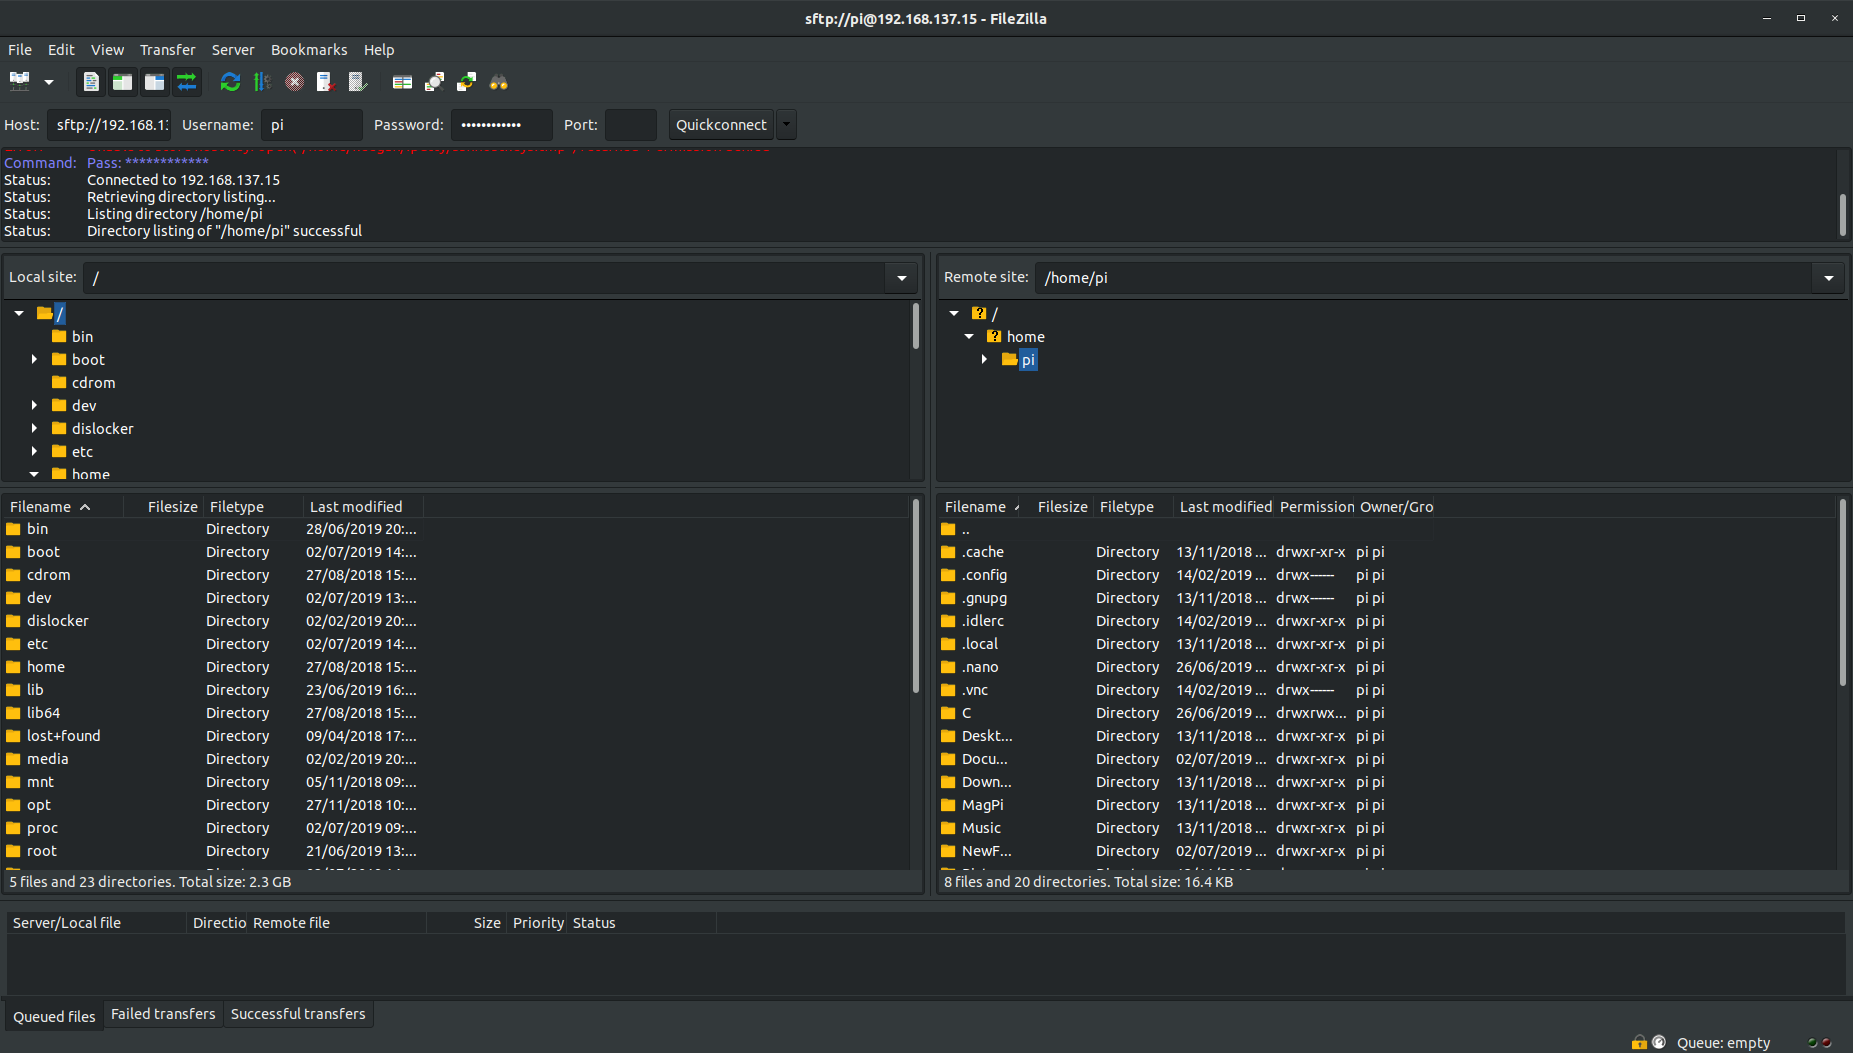
\includegraphics[width=1\columnwidth]{Figures/filezilla}
\caption{The FileZilla GUI, connected to the Pi from Ubuntu 18.10}
\label{fig:filezilla}
\end{figure}